\documentclass[10pt,aspectratio=43]{beamer}

\usepackage{graphicx}
\graphicspath{{prebuilt_images/}}
\usepackage[sectionpages,
			rotationcw % clockwise, default is counterclockwise
			]{../sty/beamerthemeGlobalUniNA}

\usepackage[utf8]{inputenc}
\usepackage[english]{babel}
\usepackage[T1]{fontenc}
\usepackage{csquotes}
\usepackage{amsmath,amsfonts,amsthm,amssymb}
\usepackage{copyrightbox}

\usepackage[scaled]{beramono}
\usepackage[scale=1.05]{AlegreyaSans}
\usepackage{../sty/shortcuts_fb}
\usepackage{subcaption}
\usepackage{minted}

\usetikzlibrary{spy}
\usepackage[round]{natbib}
\bibliographystyle{plainnat}


%%%%%%%%%%%%%%%%%%%%%%%%%%%%%%%%%%%%%%%%%%%%%%%%%%%%%%%%%%%%%%%%%%%%%%%%%%%%%%%
% footnote setting: (1), (2), etc.
\usepackage{fnpct}

% Configure style for custom doubled line
\newcommand*{\doublerule}{\hrule width \hsize height 1pt \kern 0.5mm \hrule width \hsize height 2pt}

% Configure function to fill line with doubled line
\newcommand\doublerulefill{\leavevmode\leaders\vbox{\hrule width .1pt\kern1pt\hrule}\hfill\kern0pt }


\newcommand{\mytheorem}[2]{
\doublerulefill\ \framebox{\textbf{#1}}\ \doublerulefill
\vspace{0.1cm}

#2

\doublerulefill
}

\definecolor{javared}{rgb}{0.6,0,0} % for strings
\definecolor{javagreen}{rgb}{0.25,0.5,0.35} % comments
\definecolor{javapurple}{rgb}{0.5,0,0.35} % keywords
\definecolor{javadocblue}{rgb}{0.25,0.35,0.75} % javadoc
\definecolor{marron}{rgb}{0.64,0.16,0.16}
\definecolor{orange_js}{RGB}{230,159,0}

\newcommand{\mybold}[1]{\textcolor{marron}{\textbf{#1}}}
\newcommand{\cRm}[1]{\textsc{\romannumeral #1}}


%%%%%%%%%%%%%%%%%%%%%%%%%%%%%%%%%%%%%%%%%%%%%%%%%%%%%%%%%%%%%%%%%%%%%%%%%%%%%%%
%%%%%%%%%%%%%%%%%%%%%%%%%%%%%%%%%%%%%%%%%%%%%%%%%%%%%%%%%%%%%%%%%%%%%%%%%%%%%%%
% HEADER
%%%%%%%%%%%%%%%%%%%%%%%%%%%%%%%%%%%%%%%%%%%%%%%%%%%%%%%%%%%%%%%%%%%%%%%%%%%%%%%
%%%%%%%%%%%%%%%%%%%%%%%%%%%%%%%%%%%%%%%%%%%%%%%%%%%%%%%%%%%%%%%%%%%%%%%%%%%%%%%

\title[] %shown at the top of frames
{Ridge regularization: an essential concept in data science} %shown in title frame
\subtitle{Based on the article of Trevor Hastie 2020}

\date{04-2021} % explicitly set date instead of \today

\author[]%shown at the top of frames
{%shown in title frame
    {Bascou Florent} \\%
	{Lefort Tanguy}%
}

\institute[
]
{% is placed on the bottom of the title page
    University of Montpellier
}

\titlegraphic{% logos are put at the bottom-right part of the page
    
\includegraphics[width=2cm]{Logo.pdf}~ % also support multi-logos
    %
\includegraphics[width=2cm]{Logo.pdf}~ % up to 3 (after it gets messy)
    %
\includegraphics[width=2cm]{Logo.pdf} % if more, combine them in one image.
}

% You can also move it to where you want.
% This displays 3 logos above the title to the left-center-right
%\titlegraphic{%
%  \begin{picture}(0,0)
%    \put(18,165){\makebox(0,0)[rt]{
\includegraphics[width=2cm]{Logo.pdf}
%    \hspace{8em}
\includegraphics[width=2cm]{Logo.pdf}
%    \hspace{8em}
\includegraphics[width=2cm]{Logo.pdf}}}
%  \end{picture}}

\setbeamercolor{itemize subitem}{fg=red}
\setbeamertemplate{itemize subitem}[triangle]

%%%%%%%%%%%%%%%%%%%%%%%%%%%%%%%%%%%%%%%%%%%%%%%%%%%%%%%%%%%%%%%%%%%%%%%%%%%%%%%
%%%%%%%%%%%%%%%%%%%%%%%%       PLAN      %%%%%%%%%%%%%%%%%%%%%%%%%%%%%%%%%%%%%%
%%%%%%%%%%%%%%%%%%%%%%%%%%%%%%%%%%%%%%%%%%%%%%%%%%%%%%%%%%%%%%%%%%%%%%%%%%%%%%%

\begin{document}
\maketitle


%%%%%%%%%%%%%%%%%%%%%%%%%%%
% Table of contents
%%%%%%%%%%%%%%%%%%%%%%%%%%%
\begin{frame}{Content}{}
    \tableofcontents
\end{frame}

\section*{Introduction}

%%%%%%%%%%%%%%%%%%%%%%
% Presentation - OLS problem
%%%%%%%%%%%%%%%%%%%%%%
\begin{frame}{Ridge \footnote[frame]{\citet{Tikhonov43,Hoerl_Kennard70}} regularization}{Why use it?}
    Ordinary least squares:
    \[\hat\beta = \argmin_{\beta} \|y-X\beta\|_2^2 \Longleftrightarrow \hat \beta = (X^\top X)^{-1}X^\top y\]

    Problems that can happen:
    \begin{itemize}
        \item $X^\top X$ may be ill conditioned ($\kappa = \frac{\text{largest singular value}}{\text{smallest singular value}} \gg $ )
        \begin{onlyenv}<2->
            \begin{itemize}
                \item \color{red}{ Shift spectrum by $\lambda$ using $X^\top X + \lambda \mathrm{Id}.$}
            \end{itemize}
        \end{onlyenv}
        \item $p > n$ leads to infinite number of solutions for OLS.
        \begin{onlyenv}<2->
            \begin{itemize}
                \item \color{red}{ Add penalty to recover unicity.}
            \end{itemize}
        \end{onlyenv}
    \end{itemize}
    \begin{onlyenv}<3->
    \begin{block}{Ridge estimator}
        \[ \hat\beta_{ridge} = \argmin_{\beta} \|y-X\beta\|_2^2 \textcolor{red}{+ \lambda \|\beta\|^2_2} \Longleftrightarrow \hat \beta = (X^\top X \textcolor{red}{+ \lambda \mathrm{Id}})^{-1}X^\top y \]
    \end{block}
    \end{onlyenv}
\end{frame}


\begin{frame}{Ridge regularization}{Some generalities}
    \begin{onlyenv}<1->
    \begin{itemize}
        \item<1-> Coefficients with smaller $\ell_2$ norm,
        \item<1-> Handles the multicolinearity issue,
        \item<1-> Don't apply only to linear models, in general:
        \[\argmin_w f(w) + \lambda \|w\|^2_2 \enspace.\]
    \end{itemize}
\end{onlyenv}
\begin{onlyenv}<2->
        \begin{block}{Some cons (because there must be some)}
            \begin{itemize}
        \item<2-> Alone won't give sparse solutions, $\dots$
        \item<2-> \textbf{BUT} can be combined with a LASSO\only<2->\footnote[frame]{\citet{Tibshirani96}} which gives the Elastic-Net \only<2->\footnote[frame]{\citet{Zou_Hastie05}}:
        \[\argmin_\beta \|y-X\beta\|_2^2 + \lambda_1 \|\beta\|_1 + \lambda_2 \|\beta\|_2^2\enspace.\]
        \item<2-> Introduce an hyperparameter that needs tuning.
            \end{itemize}
        \end{block}
    \end{onlyenv}
\end{frame}

\begin{frame}{Different penalties}{And different shapes}
    \begin{figure}
        \centering
        \copyrightbox[b]{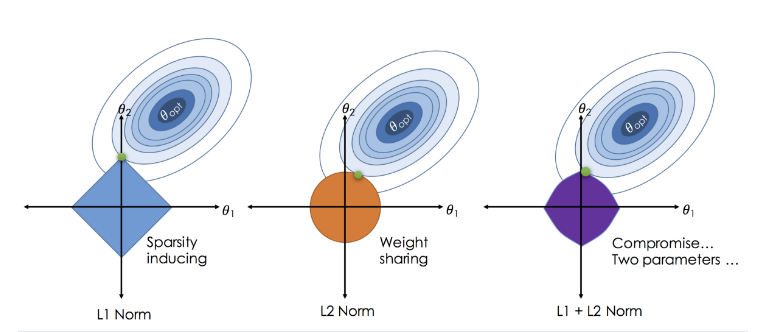
\includegraphics[scale=.4]{balls_reg.png}
        }%
           {Source: \url{https://towardsdatascience.com/}}
    \end{figure}

\end{frame}

%%%%%%%%%%%%%%%%%%%%%%%%
% Ridge computation, SVD and LOO CV
%%%%%%%%%%%%%%%%%%%%%%%%
\section{Ridge computational cost}
\begin{frame}{Ridge estimator}{How to compute it efficiently}
    Solution is given by : $ \hat \beta_{\lambda} = (X^\top X \textcolor{red}{+ \lambda \mathrm{Id}})^{-1}X^\top y$
    \\
    % In many applications, $\lambda$ is a tuning parameters leading to computing a number of solution of $\beta_{ridge}$
    Problem : $\lambda$ is a tuning parameter $\Longrightarrow$ computing many $\hat \beta_{\lambda}$
    % \begin{itemize}
    %     \item $\lambda$ is a tuning parameter $\Rightarrow$ computing many solution of $\hat \beta_{\lambda}$
    % \end{itemize}
   \begin{onlyenv}<2->
        \begin{block}{Use ONE SVD ($X = U D V^\top$) to compute many estimations}
        % Use SVD (singular value decomposition) to compute efficiently many solution :
        %\begin{align*}
        $$    \hat \beta_{\lambda} = (X^\top X \textcolor{red}{+ \lambda \mathrm{Id}})^{-1}X^\top y
            = V(D^\top D \textcolor{red}{+ \lambda \mathrm{Id}})^{-1}D^\top U^\top y
            = \sum_{i=1}^{rg(X)} v_j \frac{d_j}{d_j^2 + \lambda} \langle u_j \vert y \rangle $$
        % \end{align*}
        \end{block}
    \end{onlyenv}
    \begin{onlyenv}<3->
        \begin{block}{Use ONE SVD ($X = U D V^\top$) to compute many predictions}
        % Use SVD (singular value decomposition) to compute efficiently many solution :
        %\begin{align*}
        $$ \hat y_\lambda  = X \hat \beta_{\lambda} %= (X^\top X \textcolor{red}{+ \lambda \mathrm{Id}})^{-1}X^\top y
        %= U D V^\top V(D^\top D \textcolor{red}{+ \lambda \mathrm{Id}})^{-1}D^\top U^\top y
        = U D (D^\top D \textcolor{red}{+ \lambda \mathrm{Id}})^{-1}D^\top U^\top y
        = \sum_{i=1}^{rg(X)} u_j \frac{d_j^2}{d_j^2 + \lambda} \langle u_j \vert y \rangle $$
        % \end{align*}
        \end{block}
    \end{onlyenv}
    % TO DO : add equation 10 du papier puis la LOOCV sur une autre slide
\end{frame}


\begin{frame}{Ridge estimator}{LOO CV}
    Let us denote :
    \begin{itemize}
        \item $\hat \beta_\lambda^{(-i)}$ the estimated coefficients without using the pair $(x_i, y_i)$.
        \item $R^\lambda =  X(X^\top X + \lambda \mathrm{Id})X^\top$ the Ridge operator matrix
    \end{itemize}
    \begin{onlyenv}<2>
        \begin{block}{Easy computation for LOO-CV}
        $$ LOO_\lambda
        = \sum_{i=1}^n (y_i - x_i^\top \hat \beta_\lambda^{(-i)} )^2
        = \sum_{i=1}^n \frac{(y_i - x_i^\top \hat \beta_\lambda)^2}{(1 - R^\lambda_{ii})^2} $$
        \end{block}
    \end{onlyenv}
    \begin{onlyenv}<3->
        \begin{block}{Easy computation for LOO-CV}
        $$ LOO_\lambda
            = \sum_{i=1}^n (y_i - x_i^\top \hat \beta_\lambda^{(-i)} )^2
            = \sum_{i=1}^n \frac{(y_i - x_i^\top \hat \beta_\lambda)^2}{(1 - R^\lambda_{ii})^2} $$

        $$ R^\lambda
        =  X(X^\top X + \lambda \mathrm{Id})^{-1}X^\top
        = UD(D^\top D + \lambda \mathrm{Id})^{-1} D^\top U
        = U S(\lambda) U$$
        \center{with $S(\lambda)$ the diagonal shrinkage matrix with elements $\frac{d_j^2}{d_j^2 + \lambda}$}
        \end{block}
    \end{onlyenv}
\end{frame}

\begin{frame}{Ridge estimator}{Bias and Variance}
    % As other regularized model, Ridge coefficients are shrunk toward the origin.
    Suppose that the data arises from a linear model with \emph{i.i.d} centered errors $\varepsilon_i$
    $$ y_i = x_i^\top \beta + \varepsilon_i, \quad i=1, \dots, n$$
    Then, the Ridge estimate $\hat \beta_{\lambda}$ is a biased estimate of $\beta$.
    \begin{onlyenv}<2->
        \begin{block}{Bias}
            If the $x_i$ are assumed fixed, $n > p$ and $X$ has full column rank, we get :
            $$ \mathrm{Bias}(\hat \beta_\lambda) = \sum_{j=1}^p v_j \frac{\lambda}{d_j^2 + \lambda} \langle v_j \vert \beta \rangle $$
        \end{block}
        The smaller the $j^{th}$ singular value is, the bigger the shrinkage associated is.
    \end{onlyenv}
\end{frame}

\begin{frame}{Ridge estimator}{An example of LOO CV and biais}
    % TO DO : change the data description
    \begin{onlyenv}<1>
        \begin{columns}
            \begin{column}{0.4\textwidth}
                \begin{itemize}
                    \item Isotropic data: $X\sim\mathcal{N}(0,\mathrm{Id})$,
                    \item[]
                    \item $n=50$, $p=10$
                    \item[]
                    \item \textcolor{red}{$\SNR=1$}
                    \item[]
                    \item $y = X\beta^*+\varepsilon$ with $\varepsilon\sim \mathcal{N}(0, \sigma^2\mathrm{Id})$
                \end{itemize}
            \end{column}
            \begin{column}{0.7\textwidth}
                \begin{center}
                        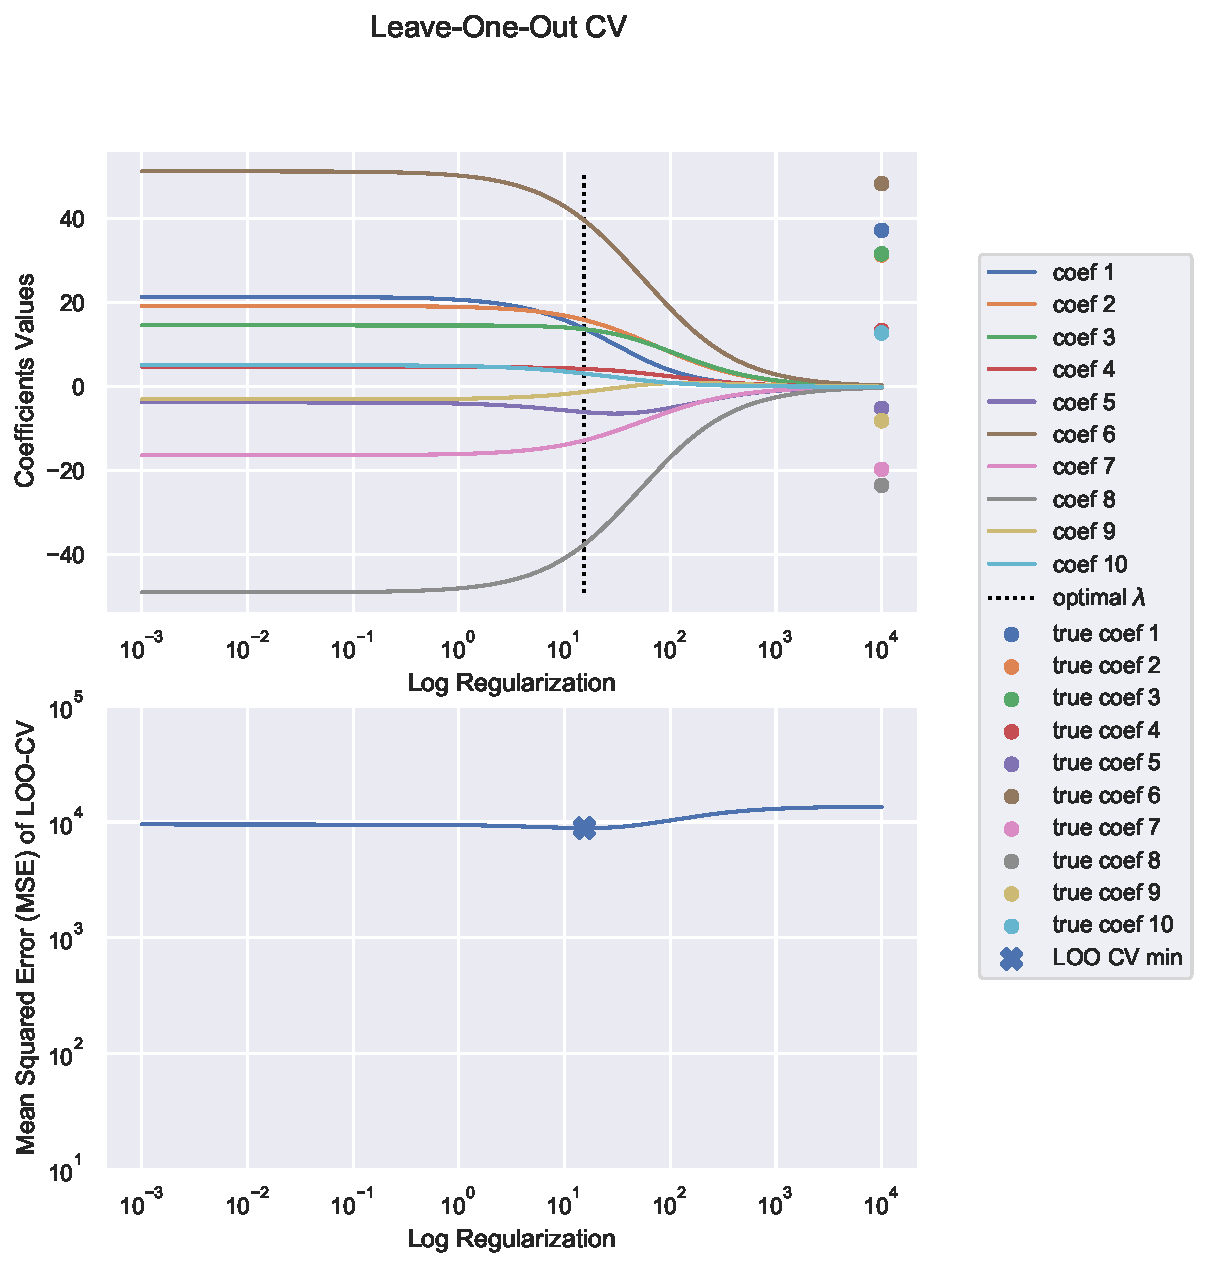
\includegraphics[width=0.95\textwidth]{path_ridge_complete_1_.pdf}
                 \end{center}
            \end{column}
            \end{columns}
    \end{onlyenv}
    \begin{onlyenv}<2>
        \begin{columns}
            \begin{column}{0.4\textwidth}
                \begin{itemize}
                    \item Isotropic data: $X\sim\mathcal{N}(0,\mathrm{Id})$,
                    \item[]
                    \item $n=50$, $p=10$
                    \item[]
                    \item \textcolor{red}{$\SNR=2$}
                    \item[]
                    \item $y = X\beta^*+\varepsilon$ with $\varepsilon\sim \mathcal{N}(0, \sigma^2\mathrm{Id})$
                \end{itemize}
            \end{column}
            \begin{column}{0.7\textwidth}
                \begin{center}
                        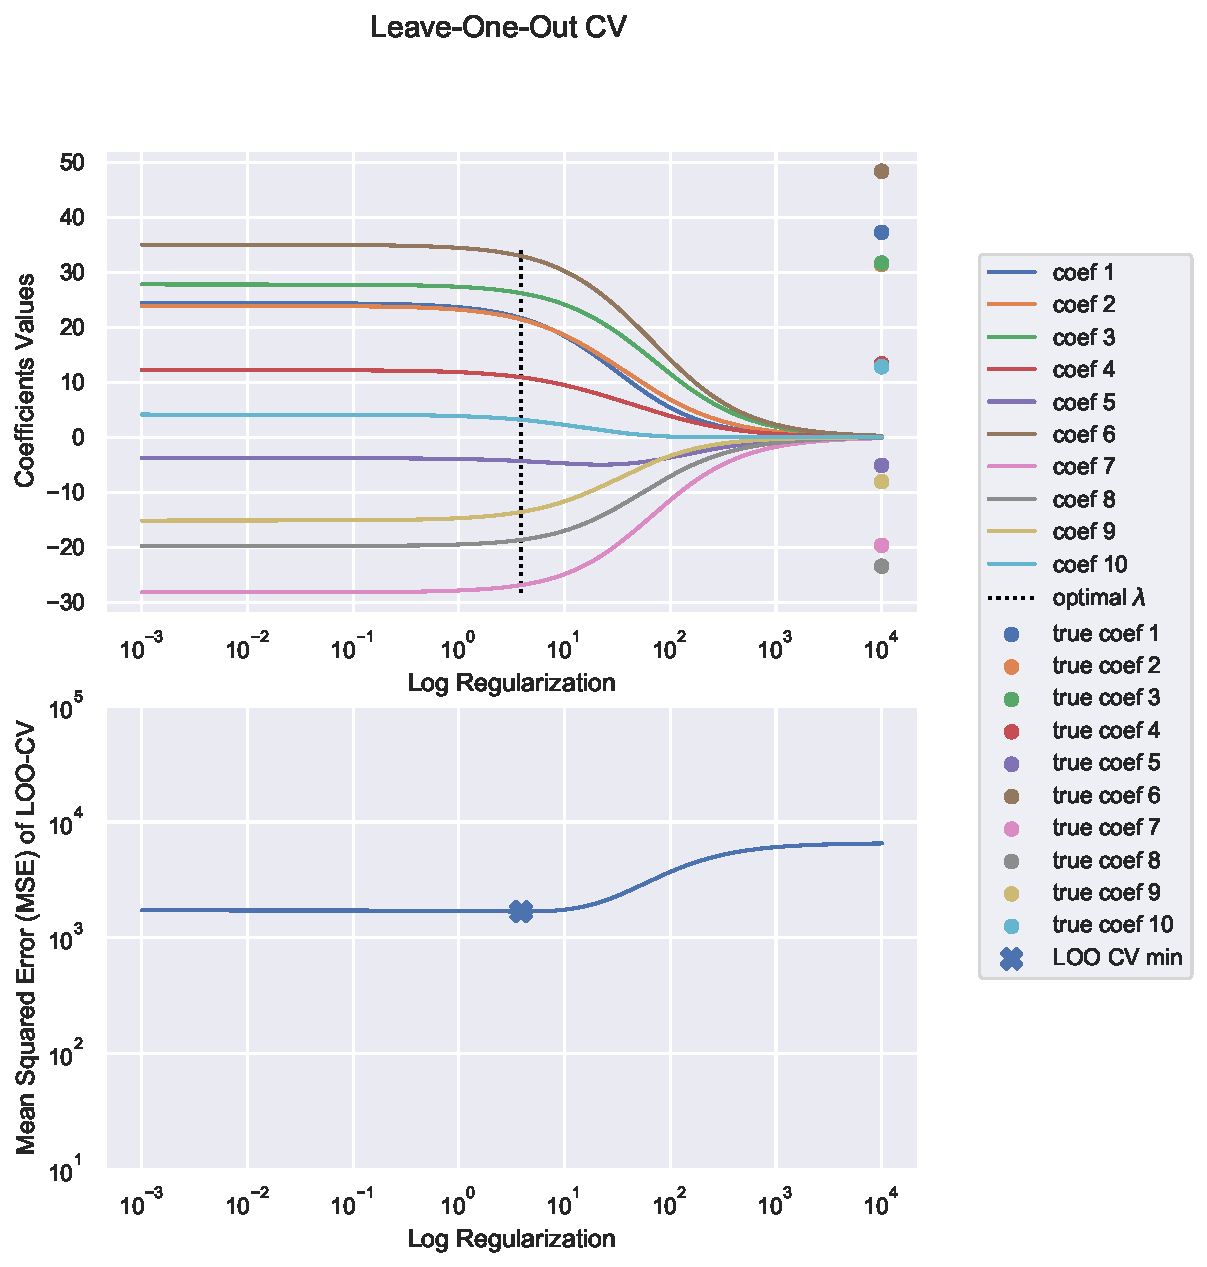
\includegraphics[width=0.95\textwidth]{path_ridge_complete_2_.pdf}
                 \end{center}
            \end{column}
            \end{columns}
    \end{onlyenv}
    \begin{onlyenv}<3>
        \begin{columns}
            \begin{column}{0.4\textwidth}
                \begin{itemize}
                    \item Isotropic data: $X\sim\mathcal{N}(0,\mathrm{Id})$,
                    \item[]
                    \item $n=50$, $p=10$
                    \item[]
                    \item \textcolor{red}{$\SNR=3$}
                    \item[]
                    \item $y = X\beta^*+\varepsilon$ with $\varepsilon\sim \mathcal{N}(0, \sigma^2\mathrm{Id})$
                \end{itemize}
            \end{column}
            \begin{column}{0.7\textwidth}
                \begin{center}
                        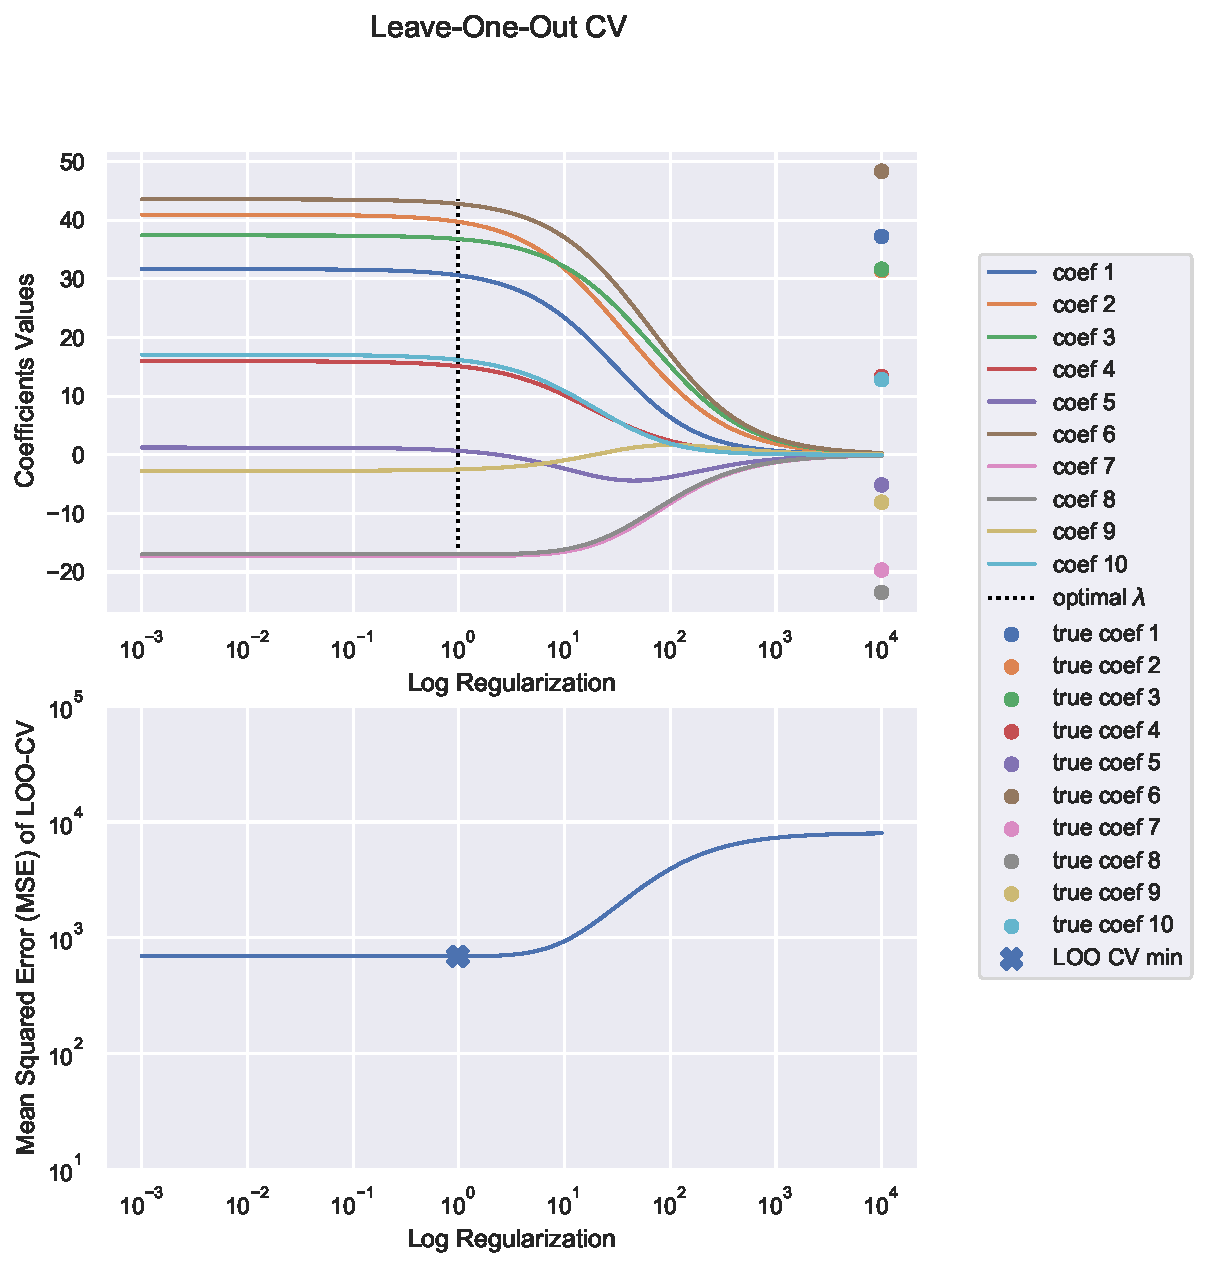
\includegraphics[width=0.95\textwidth]{path_ridge_complete_3_.pdf}
                 \end{center}
            \end{column}
            \end{columns}
    \end{onlyenv}
    \begin{onlyenv}<4>
        \begin{columns}
            \begin{column}{0.4\textwidth}
                \begin{itemize}
                    \item Isotropic data: $X\sim\mathcal{N}(0,\mathrm{Id})$,
                    \item[]
                    \item $n=50$, $p=10$
                    \item[]
                    \item \textcolor{red}{$\SNR=5$}
                    \item[]
                    \item $y = X\beta^*+\varepsilon$ with $\varepsilon\sim \mathcal{N}(0, \sigma^2\mathrm{Id})$
                \end{itemize}
            \end{column}
            \begin{column}{0.7\textwidth}
                \begin{center}
                        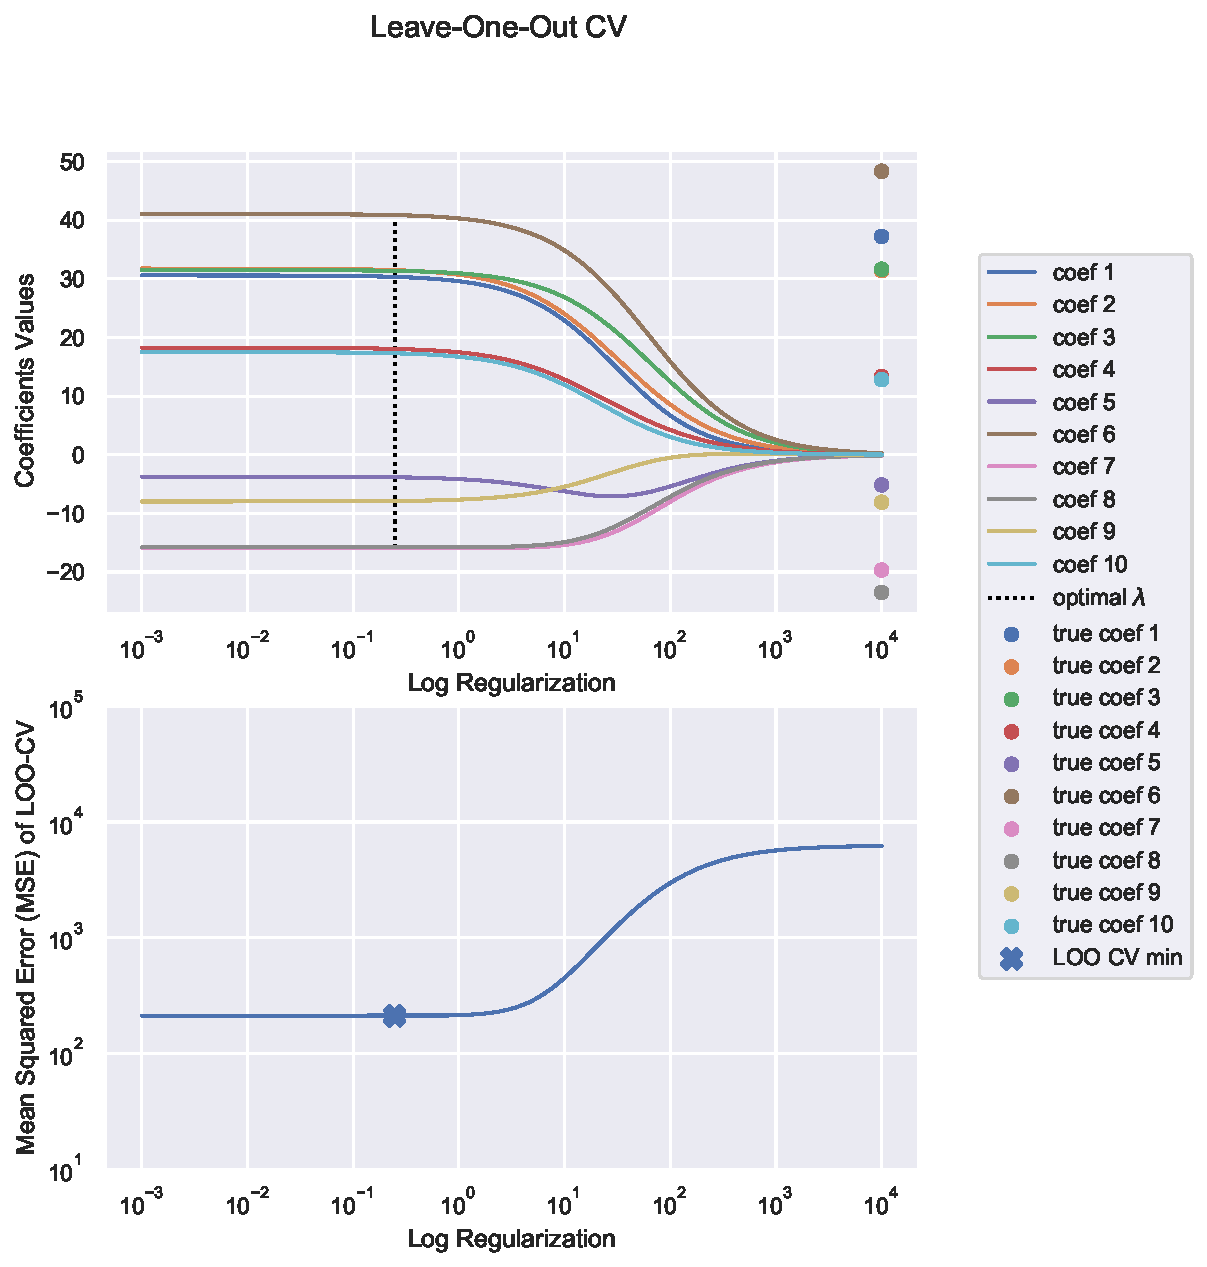
\includegraphics[width=0.95\textwidth]{path_ridge_complete_5_.pdf}
                 \end{center}
            \end{column}
            \end{columns}
    \end{onlyenv}
    \begin{onlyenv}<5>
        \begin{columns}
            \begin{column}{0.4\textwidth}
                \begin{itemize}
                    \item Isotropic data: $X\sim\mathcal{N}(0,\mathrm{Id})$,
                    \item[]
                    \item $n=50$, $p=10$
                    \item[]
                    \item \textcolor{red}{$\SNR=7$}
                    \item[]
                    \item $y = X\beta^*+\varepsilon$ with $\varepsilon\sim \mathcal{N}(0, \sigma^2\mathrm{Id})$
                \end{itemize}
            \end{column}
            \begin{column}{0.7\textwidth}
                \begin{center}
                        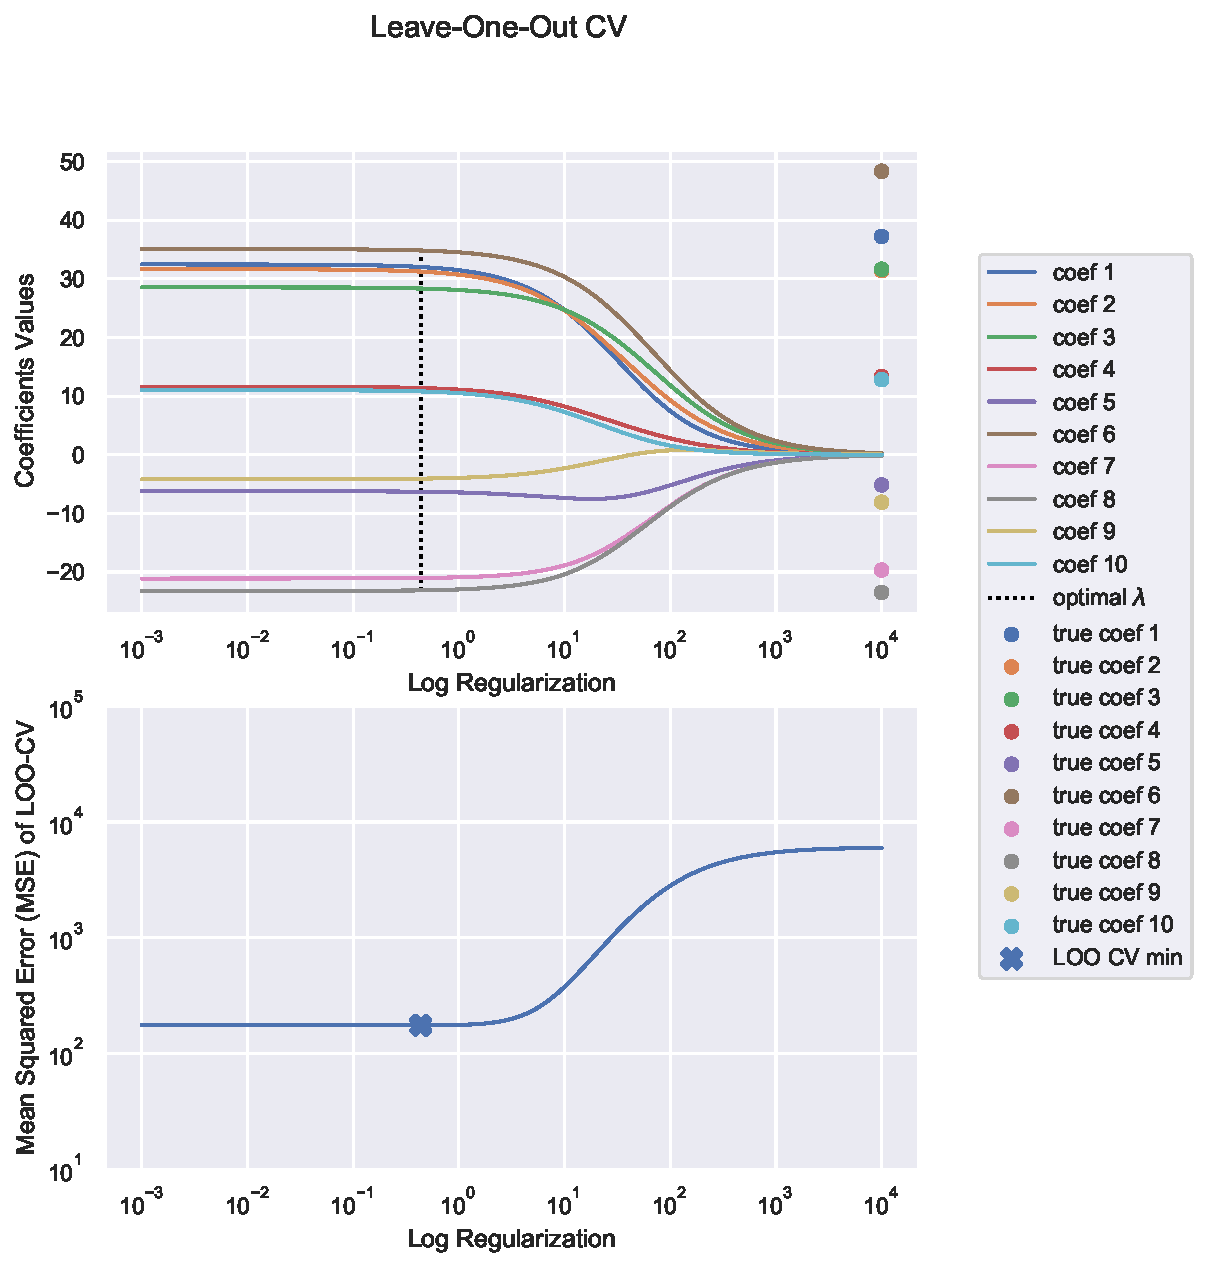
\includegraphics[width=0.95\textwidth]{path_ridge_complete_7_.pdf}
                 \end{center}
            \end{column}
            \end{columns}
    \end{onlyenv}
    \begin{onlyenv}<6>
        \begin{columns}
            \begin{column}{0.4\textwidth}
                \begin{itemize}
                    \item Isotropic data: $X\sim\mathcal{N}(0,\mathrm{Id})$,
                    \item[]
                    \item $n=50$, $p=10$
                    \item[]
                    \item \textcolor{red}{$\SNR=10$}
                    \item[]
                    \item $y = X\beta^*+\varepsilon$ with $\varepsilon\sim \mathcal{N}(0, \sigma^2\mathrm{Id})$
                \end{itemize}
            \end{column}
            \begin{column}{0.7\textwidth}
                \begin{center}
                        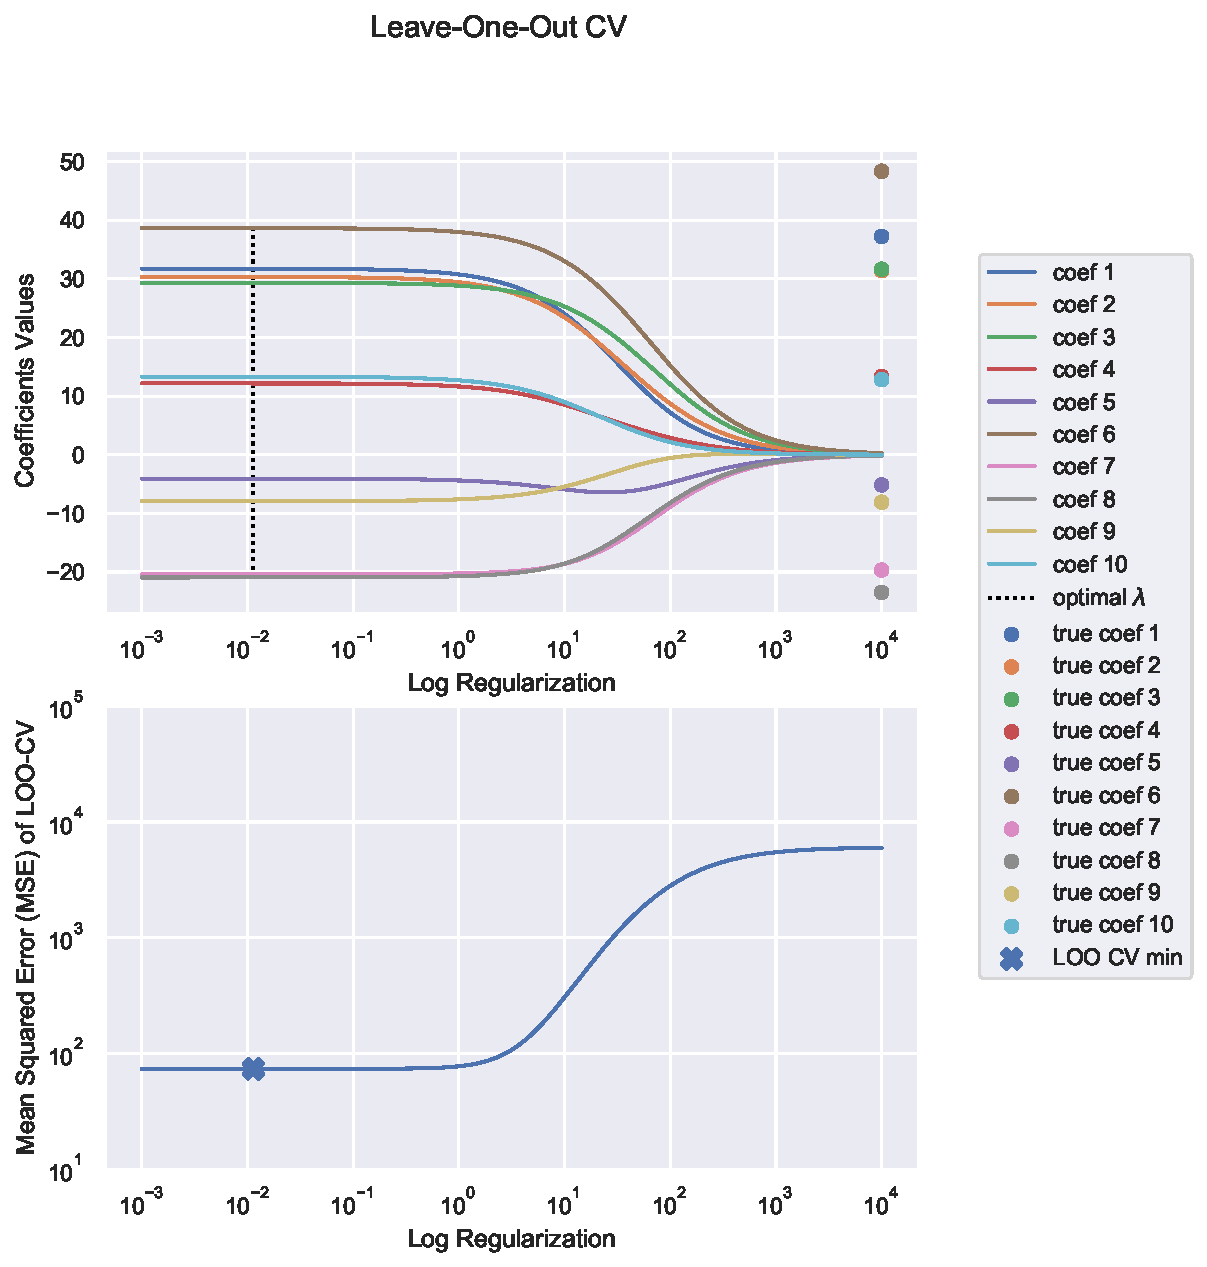
\includegraphics[width=0.95\textwidth]{path_ridge_complete_10_.pdf}
                 \end{center}
            \end{column}
            \end{columns}
    \end{onlyenv}
\end{frame}

%%%%%%%%%%%%%%%%%%%%%%%%
% Kernel trick
%%%%%%%%%%%%%%%%%%%%%%%%
\section{Kernel trick}

\begin{frame}{Kernel trick}{When doing less is better}
    \begin{block}{Reduce the complexity}
        If $p>n$, $(X^\top X + \lambda \mathrm{Id})^{-1}\in\bbR^{p\times p}$ is costly.
        But we can actually only solve a $n\times n$ system thanks to the relation \emph{(proof with SVD)}:
        \[X^\top (X X^\top + \lambda \mathrm{Id})^{-1}y = (X^\top X + \lambda \mathrm{Id})^{-1}X^\top y\enspace.\]
    \end{block}
    \pause
    So we can write $\hat \beta = X^\top u$ with $u\in\bbR^{n}$. Denote $K=XX^\top$ the \textbf{Gram} matrix,
    \begin{align*}
        \hat y &= X\hat\beta = XX^\top u \\
               &= K(K + \lambda \mathrm{Id})^{-1}y
    \end{align*}

    \begin{itemize}
        \item New ridge problem smaller to solve.
        \item \textbf{Opens the door for a lot more!}
    \end{itemize}
\end{frame}

\begin{frame}{Kernel ridge regression}{Non linear relation}
Suppose $y_i=\varphi(X_i)$, then
 $\hat\varphi = \displaystyle\argmin_{\varphi\in\mathcal{H}} \|y-\varphi(X)\|^2_2 + \lambda \|\varphi\|_\mathcal{H}\enspace.$
 \begin{block}{Representer theorem\footnote[frame]{\citet{scholkopf2001generalized}}}
        For $\mathcal{H}$ RKHS of kernel $K$ (symmetric!),
     \[\varphi = \sum_{i=1}^n \alpha_i K(x_i, \bullet)\enspace.\]
 \end{block}
 \pause
 The problem is now $\hat\alpha = \displaystyle\argmin_{\alpha} \|y-K\alpha\|^2_2 + \lambda \alpha^\top K \alpha$.
 \begin{itemize}
     \item first order conditions: $\nabla=(KK + \lambda K)\hat\alpha - Ky = 0$,
     \item solution: \[\textcolor{red}{\hat\alpha = (K+\lambda\mathrm{Id})^{-1}y} \enspace.\]
 \end{itemize}
\end{frame}


\begin{frame}{Kernel ridge regression}{Example with \texttt{KeOps} package}
    Gaussian kernel to estimate $\varphi(t) = t + t\cos(6t)$ on noised data,
\[K(x,y)=\exp\left\{-\gamma\|x - y\|^2_2\right\}, \gamma=\frac{1}{2\cdot 0.2^2} \enspace.\]
\begin{figure}
    \centering
    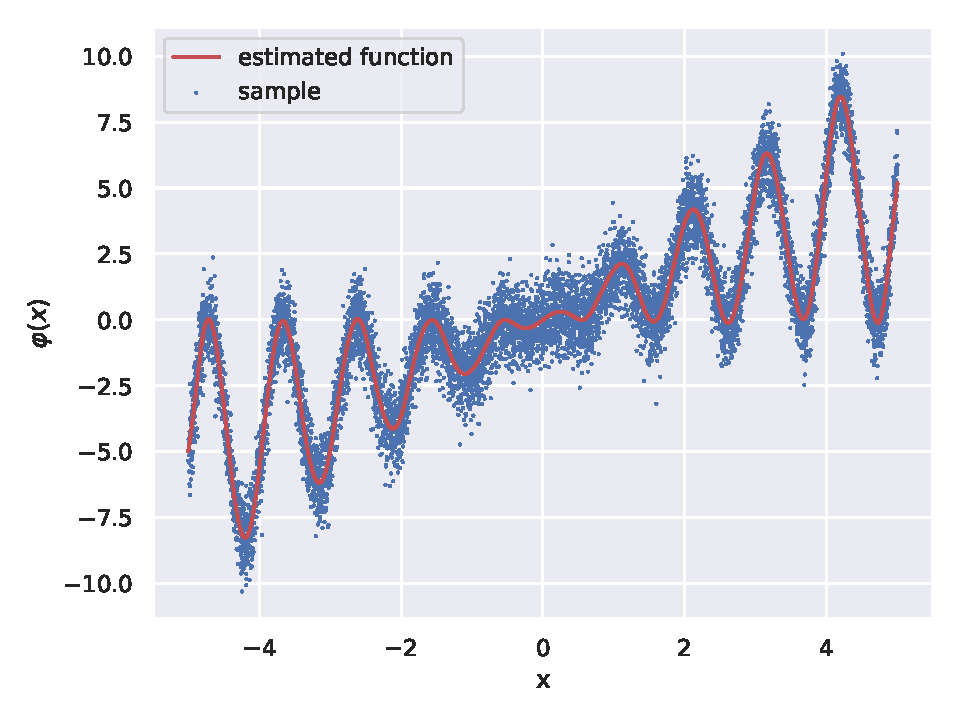
\includegraphics[scale=.45]{KRR.pdf}
\end{figure}
\end{frame}


%%%%%%%%%%%%%%%%%%%%%%%%
% Data augmentation
%%%%%%%%%%%%%%%%%%%%%%%%
\section{Data augmentation}

\begin{frame}{Data augmentation\footnote[frame]{\citet{chollet2018deep}}}{With images}
    \begin{center}
        Example of a small dog from CIFAR10 dataset
    \end{center}
    \begin{onlyenv}<1>
        \begin{figure}
            \centering
            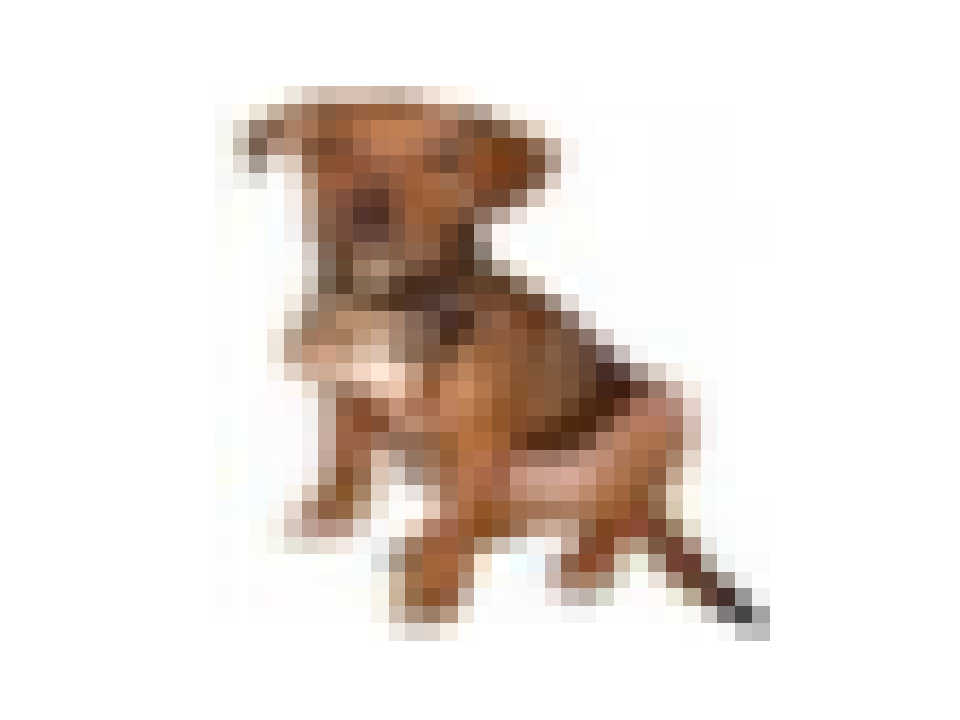
\includegraphics[scale=.6]{dog_cifar.pdf}
        \end{figure}
    \end{onlyenv}
    \begin{onlyenv}<2->
        \centering
    \begin{columns}[t]
        \column{.5\paperwidth}
        \begin{figure}
        \centering
        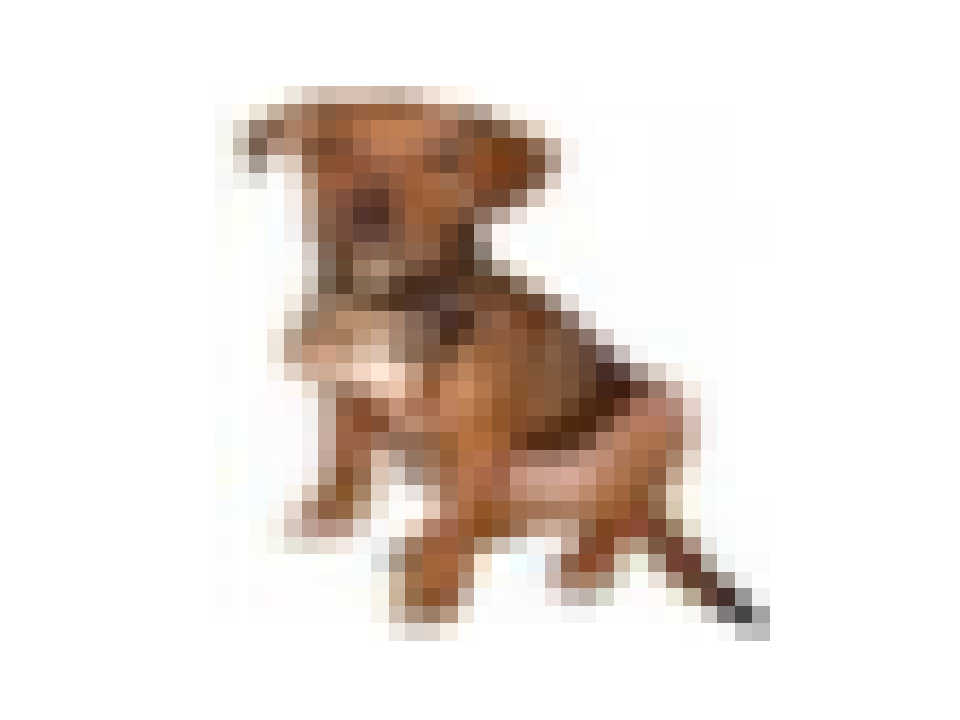
\includegraphics[scale=.4]{dog_cifar.pdf}
        \end{figure}
        \column{.5\paperwidth}
        \centering
        \begin{onlyenv}<2>
            \begin{figure}
                \reflectbox{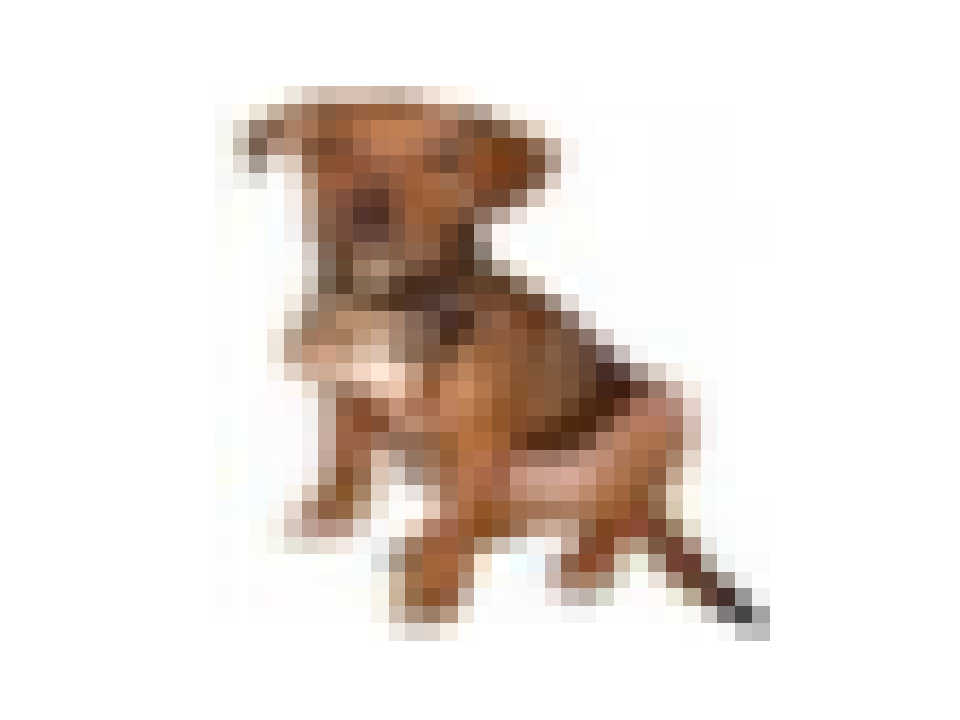
\includegraphics[scale=.4]{dog_cifar.pdf}
                }
            \end{figure}
        \end{onlyenv}
        \begin{onlyenv}<3>
            \begin{figure}
                \vspace{-1.2cm}
            \hbox{\hspace{-3em}
            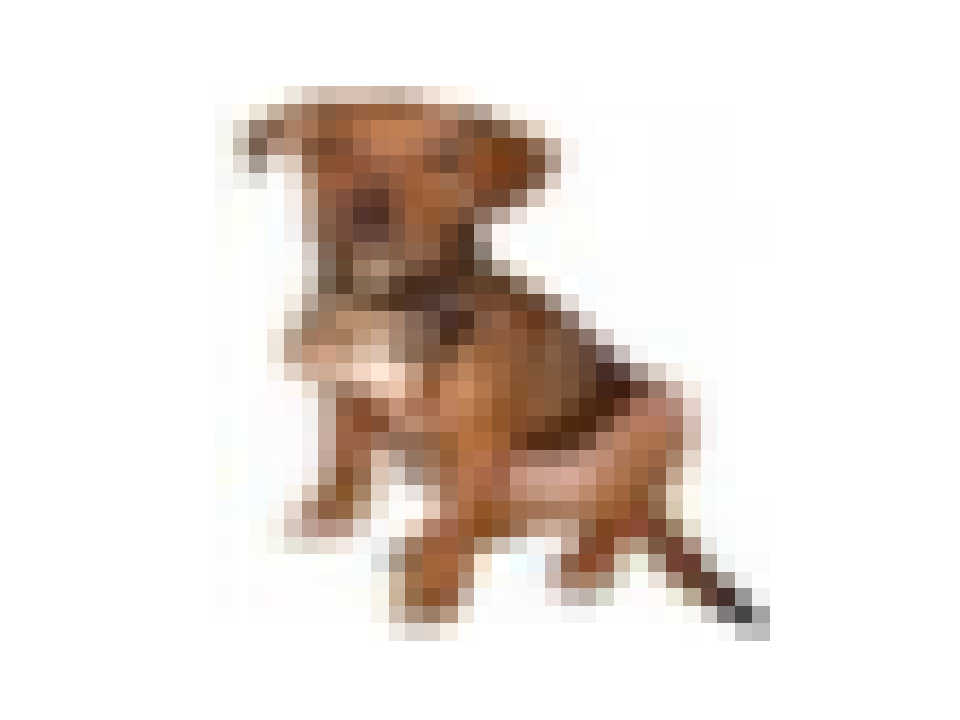
\includegraphics[scale=.4, angle=30, origin]{dog_cifar.pdf}}
            \end{figure}
        \end{onlyenv}
    \end{columns}
    \end{onlyenv}
\end{frame}

\begin{frame}{Data augmentation}{And with cloud points?}
    \begin{figure}
        \centering
        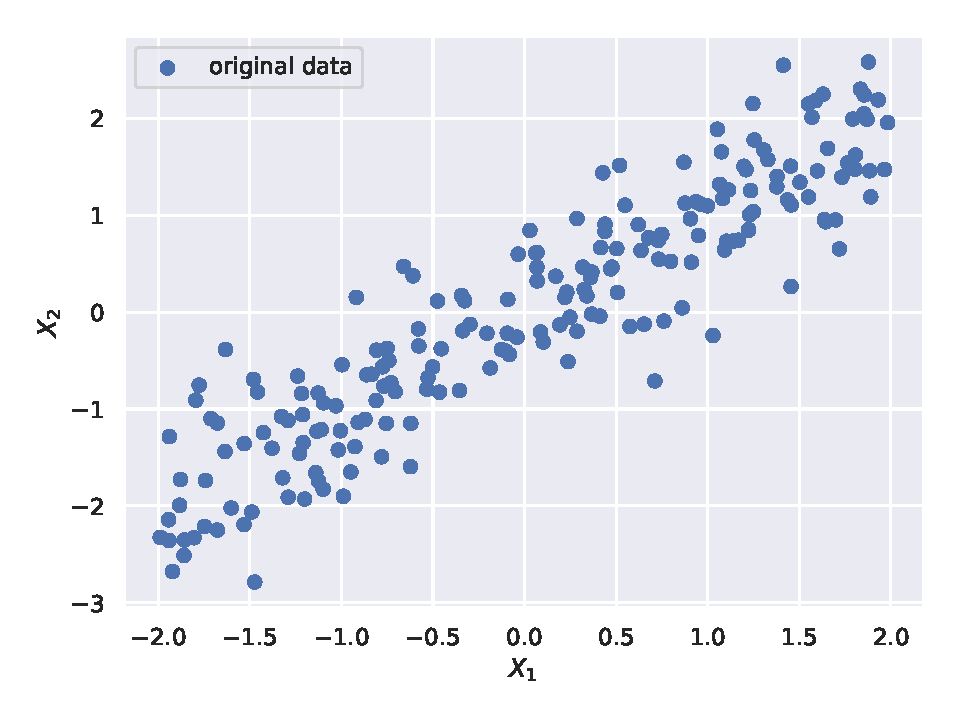
\includegraphics[scale=.5]{og_data_augm.pdf}
    \end{figure}
    \begin{itemize}
        \item \textbf{Goal:} Use the data we have to create new points,
        \item \textbf{But} can't flip it / make a small rotation, $\dots$
    \end{itemize}
\end{frame}

\begin{frame}{Data augmentation}{Perturbations on the cloud}
    One way to do so: create perturbated points from the data we have:
    \[x_{ij}=x_i + \varepsilon_{i,j}, \varepsilon_{ij}\sim\mathcal{N}\left(0, \frac{\lambda}{n}\mathrm{Id}\right), i\in[n], j\in[m]\enspace,\]
    \[\text{with associated response }y_{ij}=y_i\enspace .\]
    \vspace{-.5cm}
    \begin{columns}
        \begin{column}{.6\paperwidth}
            \begin{figure}
                \centering
                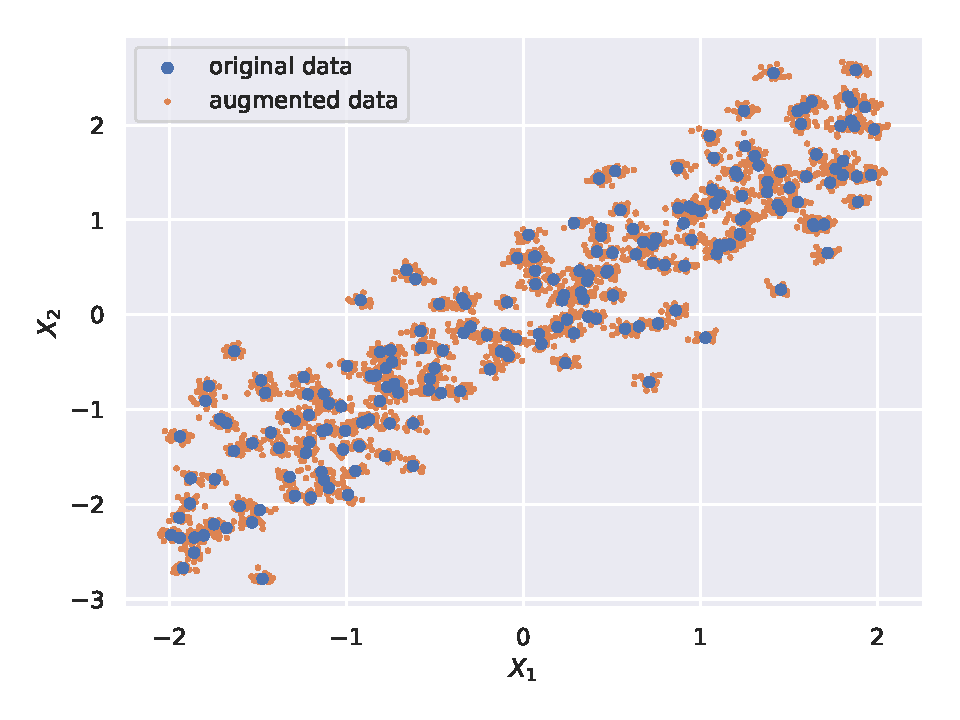
\includegraphics[scale=.35]{data_augmentation.pdf}
            \end{figure}
        \end{column}
        \begin{column}{.4\paperwidth}
            Added points compensate each other $$ \textcolor{red}{\sum_i\frac{1}{m}\sum_jx_{ij}x_{ij}^\top \simeq (XX^\top + \lambda \mathrm{Id})}$$
            OLS with $X^{augmented} \simeq$ Ridge with $X$
        \end{column}
    \end{columns}
\end{frame}

%%%%%%%%%%%%%%%%%%%%%%%%
% Dropout
%%%%%%%%%%%%%%%%%%%%%%%%
\section{Dropout regularization}
\begin{frame}{Dropout \footnote[frame]{\citet{srivastava2014dropout}}}{Randomized drop}
    \begin{itemize}
        \item Randomly set units of a layer to $0$ with probability $\phi$ to avoid overfitting,
        \item Inflate surviving ones by $1/(1-\phi)$ factor as compensation.
    \end{itemize}

    \begin{onlyenv}<1>
        \begin{figure}
            \centering
            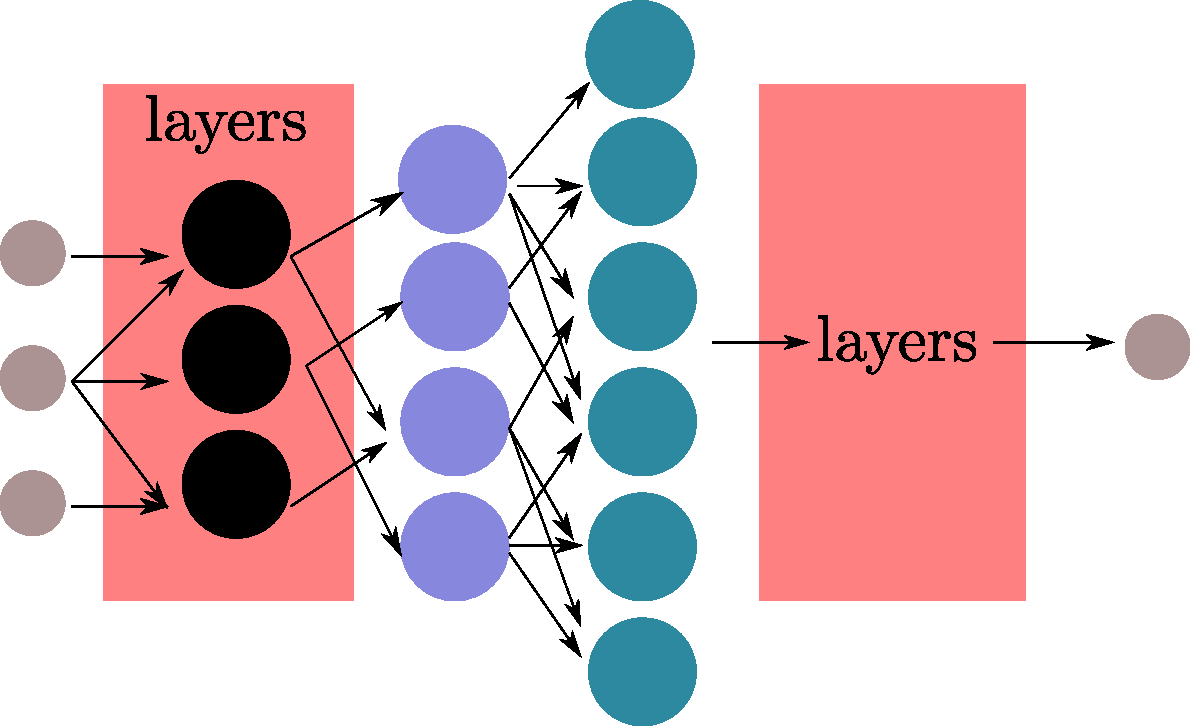
\includegraphics[scale=.4]{dropout_structure.pdf}
        \end{figure}
    \end{onlyenv}
    \begin{onlyenv}<2>
        \begin{figure}
            \centering
            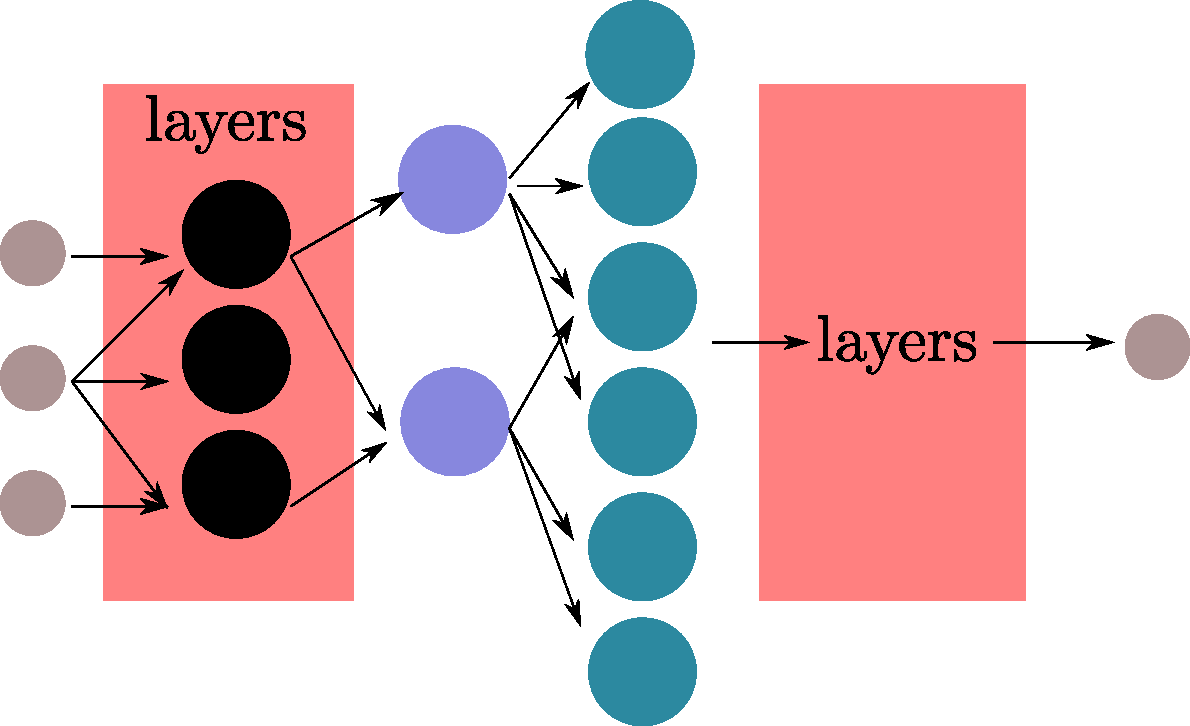
\includegraphics[scale=.4]{dropout_structure_applied.pdf}
        \end{figure}
    \end{onlyenv}

\end{frame}


\begin{frame}{Dropout}{Linear regression and Ridge  \footnote[frame]{\citet{wager2013dropout}}}
    Denoting $(I_{ij})_{ij}$ the dropout mask on $X=(x_{ij})_{ij}$ then cost function is:

    \[L(\beta) = \frac{1}{2}\sum_{i=1}^n\left(y_i - \sum_{j=1}^p x_{ij}I_{ij}\beta_j\right)^2\enspace.\]

    Note that $\bbE[I_{ij}] = 0\phi + \frac{1}{1-\phi} (1-\phi) = 1$, thus:

    \[\bbE\left[\frac{\partial}{\partial \beta}\right] = XX^\top\beta - X^\top y + \frac{\phi}{1 - \phi}\mathrm{diag}(\|x_j\|^2)_{j=1}^p\beta\enspace, \]

    \begin{onlyenv}<2->
        \begin{block}{Link with ridge}
            Solving first order conditions:
            \[\hat\beta^{dropout} = \left(X^\top X - \frac{\phi}{1 - \phi}\diag(\|x_j\|^2)\right)^{-1}X^\top y\enspace.\]
            Normalizing out data leads \textbf{in average} to the ridge estimator for $\lambda = \frac{\phi}{1 - \phi}$.
        \end{block}

    \end{onlyenv}

\end{frame}


\begin{frame}[fragile]{Dropout}{In practice with \texttt{PyTorch}}
No hastle to implement a dropout layer in a Neural Network with \texttt{PyTorch} with this inflation rate:
\begin{minted}[
    frame=lines,
    fontsize=\footnotesize,
    linenos
    ]
    {python}

class MyModel(nn.Module):
    def __init__(self, phi):
        super(MyModel, self).__init__()
        # all your great layers
        self.drop = nn.Dropout(phi)

    def forward(self, x):
        # forward x until the desired layer
        out = self.drop(current_x)
        # forward out until the output layer
        return out
\end{minted}
\end{frame}

\begin{frame}{Dropout experiment}
    With $\phi = 0.5$ (generally $0.3 \leq \phi \leq 0.5$) and $5$ repetitions:
    \begin{figure}
        \centering
        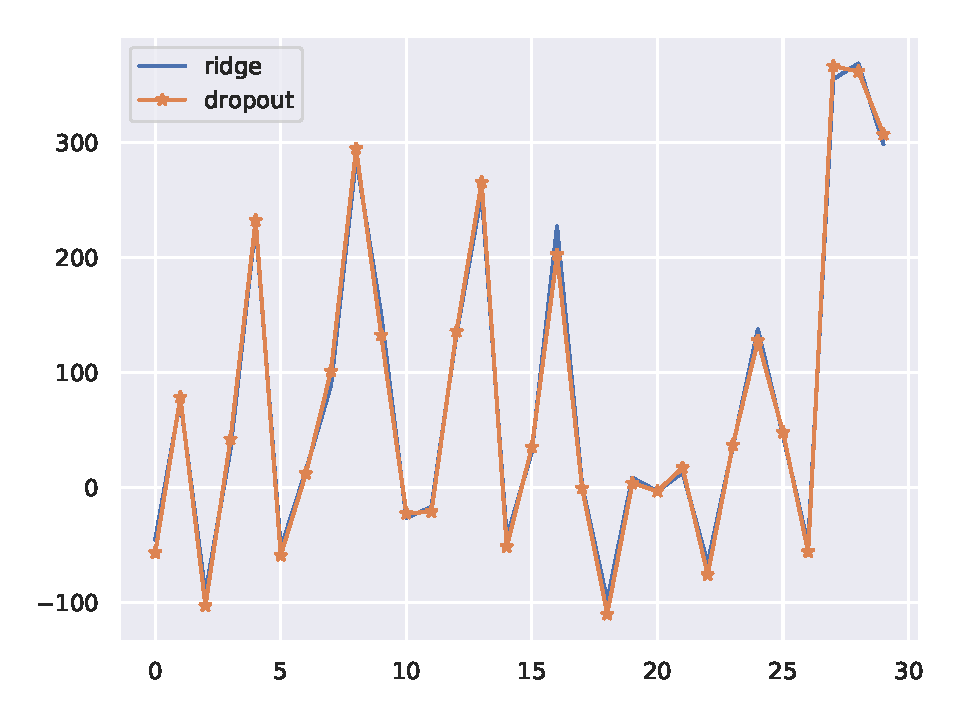
\includegraphics[scale=.5]{dropout.pdf}
        \caption{Coefficients of $\beta$ for the ridge and dropout method with $n=80, p=30$ and ridge penalty $\lambda=\phi / (1 - \phi)=1$}
    \end{figure}
\end{frame}

%%%%%%%%%%%%%%%%%%%%%%%%
% Double descent
%%%%%%%%%%%%%%%%%%%%%%%%
\section{Double descent}
\begin{frame}{Double descent}{Over parametrization}
    Phenomenon observed in Deep Learning, Random Forests \dots
    \begin{onlyenv}<1>
        \begin{figure}
            \centering
            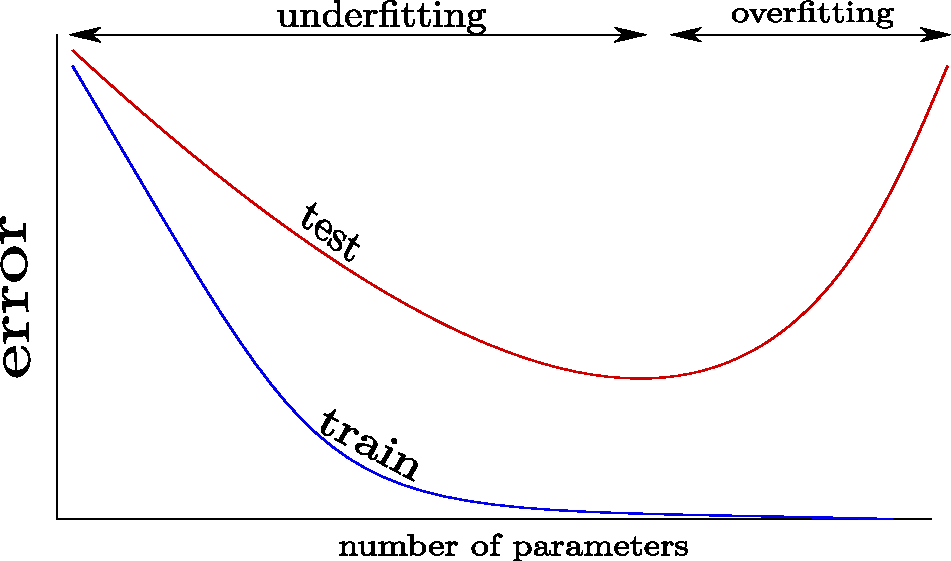
\includegraphics[scale=.6]{under_overfit_curves.pdf}
        \end{figure}
    \end{onlyenv}
    \begin{onlyenv}<2>
        \begin{figure}
            \centering
            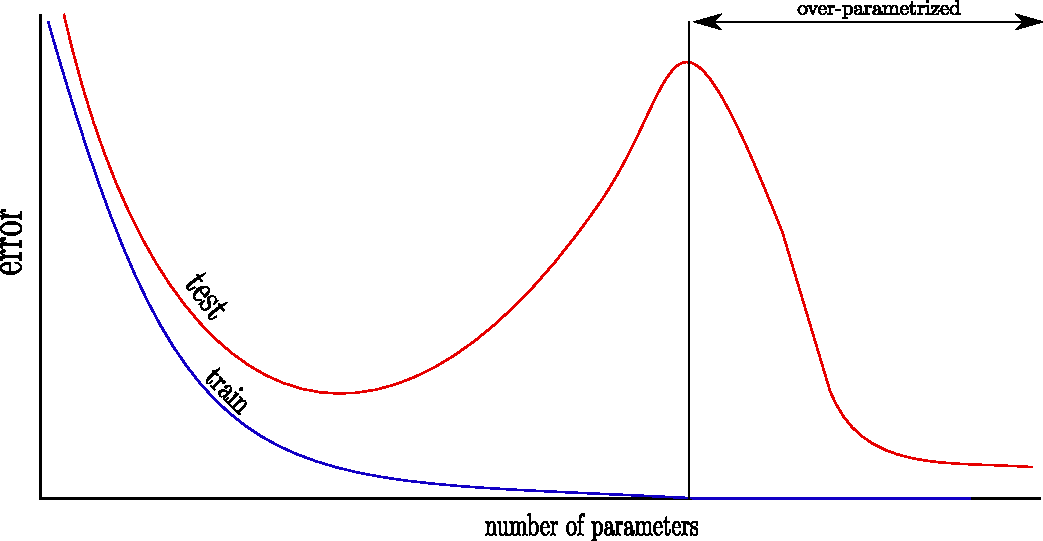
\includegraphics[scale=.6]{scheme_doubledescent.pdf}
        \end{figure}
    \begin{itemize}
        \item interpolate the data $\Longrightarrow$ $\ell_2$ norm of $\hat\beta$ is high,
        \item smaller $\ell_2$ norm for $\hat\beta$ generalizes better and we keep zero training error.
    \end{itemize}
    \end{onlyenv}
\end{frame}


%%%%%%%%%%%%%%%%%%%%%%%%
% double descent - example OLS fail
%%%%%%%%%%%%%%%%%%%%%%%%
\begin{frame}{Double descent}{Example on samples number - 25 repetitions}
    % TODO : légende figure a changer
    % Ordinary Least Square produce double descent phenomenon when train samples have the same size than the number of features.
    \begin{columns}
        \begin{column}{0.46\textwidth}
            \begin{itemize}
                \item Isotropic data: $X\sim\mathcal{N}(0,\mathrm{Id})$,
                \item[]
                \item $n=1000$, $p=200$, $\|\beta^*\|_2=1$
                % $\sigma = \frac{\sqrt{\beta^{*^\top}X^\top X \beta^{*}}}{\sqrt{n} SNR} $
                \item[]
                \item $y = X\beta^*+\varepsilon$ with $\varepsilon\sim \mathcal{N}(0, \sigma^2\mathrm{Id})$,
            \end{itemize}
        \end{column}
        \begin{column}{0.7\textwidth}
            \begin{center}
             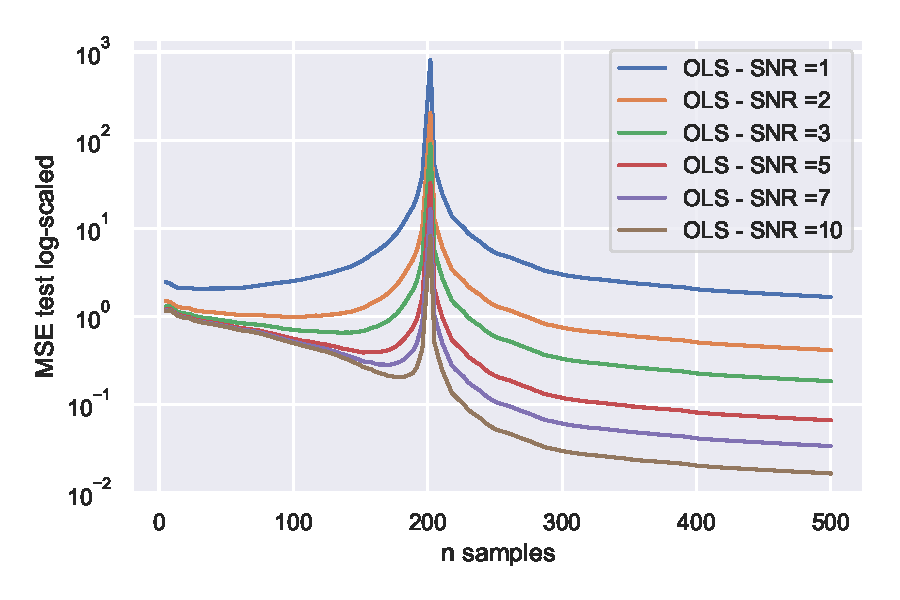
\includegraphics[width=1\textwidth]{ols_fail_log_snr.pdf}
             \end{center}
        \end{column}
        \end{columns}
    %\begin{onlyenv}<2>
        \begin{block}{}
            Ordinary Least Square produces a double descent phenomenon when training set has same size as the number of features.
        \end{block}
    %\end{onlyenv}
\end{frame}


\begin{frame}{Double descent}{Example on features number - 25 repetitions}
    % TODO : légende figure a changer
    % Ordinary Least Square produce double descent phenomenon when train samples have the same size than the number of features.
    \begin{columns}
        \begin{column}{0.46\textwidth}
            \begin{itemize}
                \item To generate data :
                \begin{itemize}
                    \item Isotropic data: $X\sim\mathcal{N}(0,\mathrm{Id})$,
                    %\item[]
                    \item $n=p=100$,
                    $\|\beta^*\|_2=1$
                    %\item[]
                    % $\sigma = \frac{\sqrt{\beta^{*^\top}X^\top X \beta^{*}}}{\sqrt{n} SNR} $
                    %\item[]
                    \item $y = X\beta^*+\varepsilon$ with $\varepsilon\sim \mathcal{N}(0, \sigma^2\mathrm{Id})$,
                \end{itemize}
                \item To learn model :
                \begin{itemize}
                    \item if $p\leq n$, use $X$ from data ;
                    \item if $p > n$, merge columns to $X$ from random distribution.
                \end{itemize}
            \end{itemize}
        \end{column}
        \begin{column}{0.7\textwidth}
            \begin{center}
             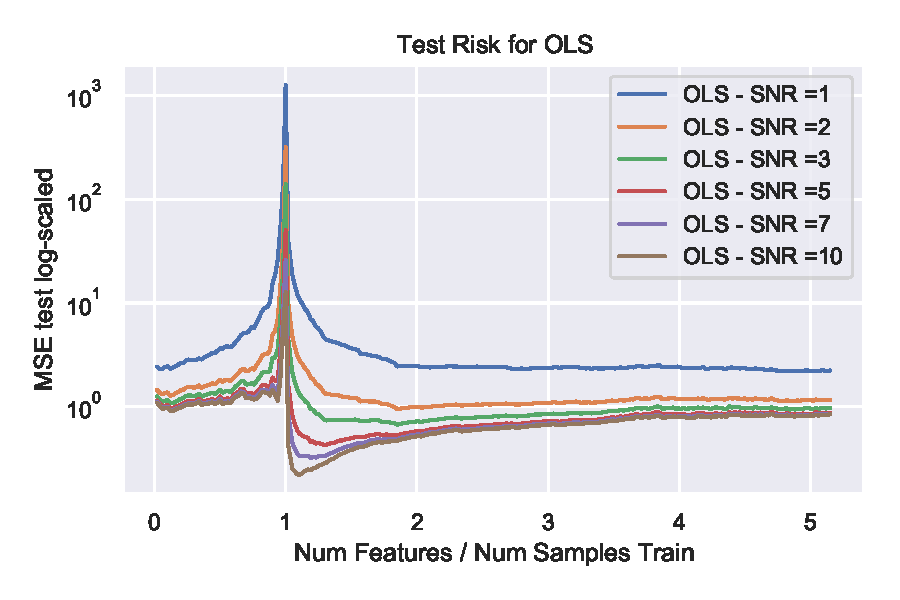
\includegraphics[width=1\textwidth]{ols_fail_log_snr_features.pdf}
             \end{center}
        \end{column}
        \end{columns}
    %\begin{onlyenv}<2>
        \begin{block}{}
            Ordinary Least Square produces a double descent phenomenon when the number of features is the same as the number of samples.
        \end{block}
    %\end{onlyenv}
\end{frame}

%%%%%%%%%%%%%%%%%%%%%%%%%%%%%%
% double descent with samples
%%%%%%%%%%%%%%%%%%%%%%%%%%%%%%

\begin{frame}{Double descent}{With samples \citep{nakkiran2020optimal} - 25 repetitions}
    In some cases ridge regularization can help get a monotonous error curve.
    \begin{columns}
        \begin{column}{0.46\textwidth}
            \begin{itemize}
                \item Isotropic data: $X\sim\mathcal{N}(0,\mathrm{Id})$,
                \item[]
                \item $n=1000$, $p=200$, $\|\beta^*\|_2=1$
                \item[]
                \item $y = X\beta^*+\varepsilon$ with $\varepsilon\sim \mathcal{N}(0, \sigma^2\mathrm{Id})$,
                \item $\lambda_{opt} = \sigma^2p$
            \end{itemize}
        \end{column}
        \begin{column}{0.7\textwidth}
            \begin{center}
             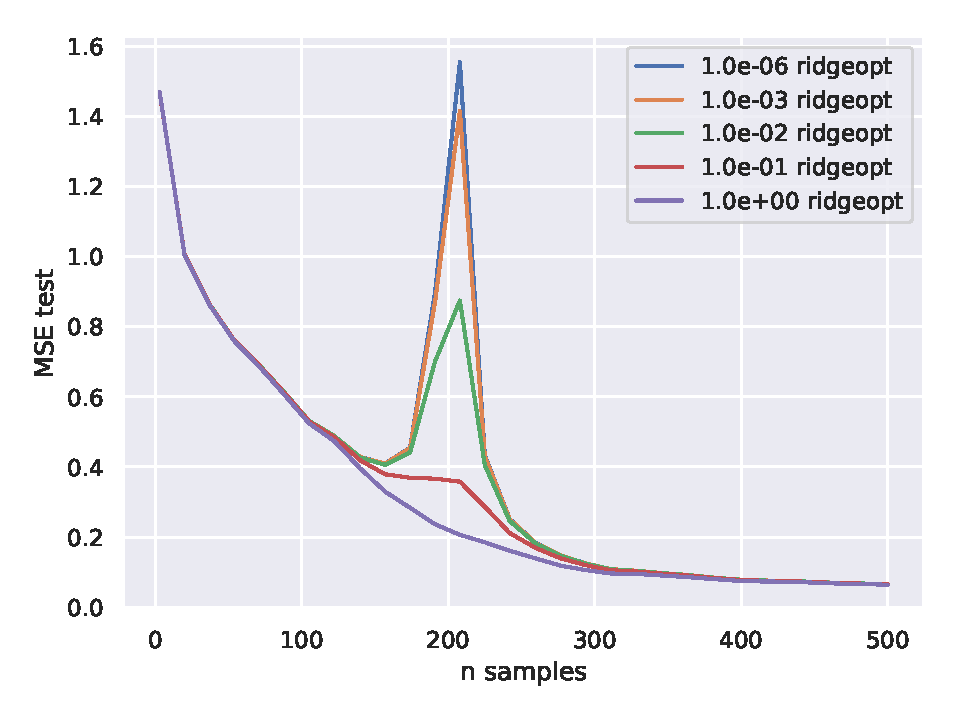
\includegraphics[width=1\textwidth]{double_descent.pdf}
             \end{center}
        \end{column}
        \end{columns}
    \begin{onlyenv}<2>
        \begin{block}{}
        We can achieve monotonic test error decrease with ridge regularization varying $p$ or $n$ for the linear models with isotropic covariates.
        \end{block}
    \end{onlyenv}
\end{frame}

\begin{frame}{Double descent}{With samples \citep{nakkiran2020optimal} - 25 repetitions}
    In some cases ridge regularization can help get a monotonous error curve.
    \begin{columns}
        \begin{column}{0.46\textwidth}
            \begin{itemize}
                \item Isotropic data: $X\sim\mathcal{N}(0,\mathrm{Id})$,
                \item[]
                \item $n=1000$, $p=200$, $\|\beta^*\|_2=1$
                \item[]
                \item $y = X\beta^*+\varepsilon$ with $\varepsilon\sim \mathcal{N}(0, \sigma^2\mathrm{Id})$,
                \item $\lambda_{opt} = \sigma^2p$
            \end{itemize}
        \end{column}
        \begin{column}{0.7\textwidth}
            \begin{center}
             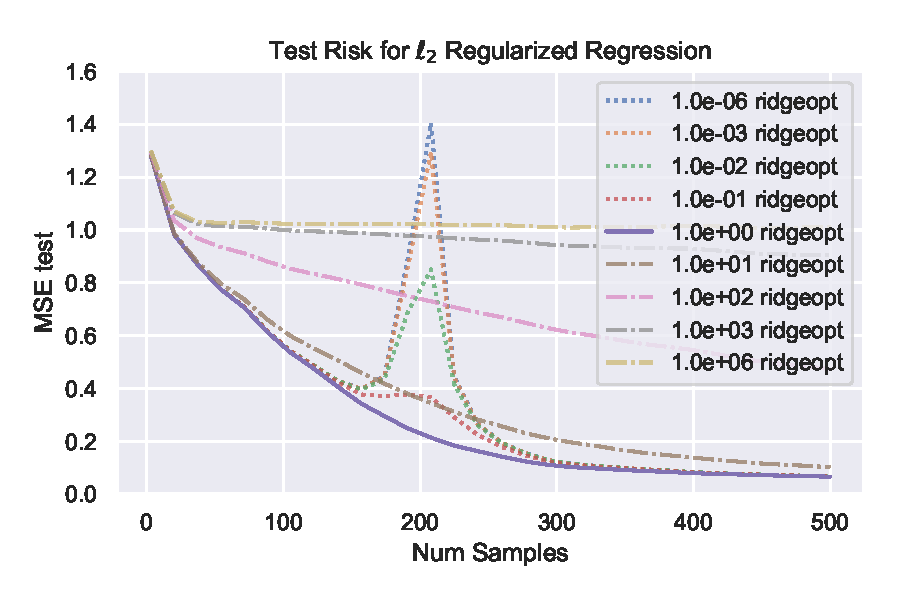
\includegraphics[width=1\textwidth]{double_descent_sup.pdf}
             \end{center}
        \end{column}
        \end{columns}
        \begin{block}{}
        This property remains true if $\lambda \geq \lambda_{opt}$ varying $n$ for the linear models with isotropic covariates.
        % We can achieve monotonic test error decrease with ridge regularization varying $p$ or $n$ for the linear models with isotropic covariates.
        \end{block}
\end{frame}

%%%%%%%%%%%%%%%%%%%%%%%%
% double ridge is lasso
%%%%%%%%%%%%%%%%%%%%%%%%
\section{Rank selection for matrix}
\begin{frame}{Rank selection for matrix problem}{}
    Suppose $X \in \mathbb{R}^{m\times n }$. Then we get the rank selection for matrix problem :
    $$\min_{M} \|X-M\|_F^2 \quad \text{s. t.} \quad  rank(M) \leq q$$.
    \begin{onlyenv}<2->
    \begin{itemize}
        \item Solution : set all the singular values of $D$ to zero, except the $q$ largest.
        \item Problem : the rank constraint makes this problem non-convex
    \end{itemize}
    \end{onlyenv}
    \begin{onlyenv}<3->
        \begin{block}{Convex relaxation \only<3->\footnote[frame]{\citet{Fazel02}}- LASSO version of rank selection matrix}
            $$\widetilde{M} = \argmin_{M} \|X-M\|_F^2 + \lambda \|M\|_*$$
            \begin{center}
                with $\|M\|_*$ denoting the nuclear norm - sum of singular values.
            \end{center}
        \end{block}
    \end{onlyenv}
    \begin{onlyenv}<4->
        \begin{itemize}
            \item Solution : soft-tresholding the singular values: $\max(d_i  -\lambda, 0)$
        \end{itemize}
        \end{onlyenv}
\end{frame}
\begin{frame}{Double Ridge Problem \footnote[frame]{\citet{srebro2005maximum}}}{}
    Let $X \in \mathbb{R}^{m\times n },~  A \in \mathbb{R}^{m\times q}$ and $B \in \mathbb{R}^{n \times q }$. We get the double ridge problem :
    $$ \widetilde{A}, \widetilde{B} =  \argmin_{A, B} \|X-AB^\top \|_F^2 + \lambda \|A \|_F^2 +\lambda \|B \|_F^2 $$
    \begin{onlyenv}<2->
        \begin{itemize}
            \item This is a $\ell_2$ bi-convex problem.
            % \item This problem as  the same solution that the $\ell_1$ convex relation problem  :
            \item The solution is the same as the $\ell_1$ convex relation problem  :
            $ \widetilde{A} \widetilde{B}^\top = \widetilde{M} $
        \end{itemize}
    \end{onlyenv}
    \begin{onlyenv}<2->
        \begin{block}{Interest in variation of theses  problems}
            If $X$ has missing-values, we can solve the \textit{matrix completion} objective :
            $$\widetilde{M} = \argmin_{M} \|P_\Omega (X-M)\|_F^2 + \lambda \|M\|_*$$
            \center{where $P_\Omega$ projects onto the observed values of $X$.}
        \end{block}
        \begin{itemize}
            \item This problem can be solved for large $X$ using double ridge problem\footnote[frame]{\citet{hastie2015matrix}}.
        \end{itemize}
    \end{onlyenv}
\end{frame}


\begin{frame}{Conclusion}
The Ridge regularization is linked to several modern techniques, sometimes hidden behind them.

\begin{itemize}
    \item LASSO methods are powerful, but \textcolor{red}{SO ARE RIDGE'S},
    \item it is easy to implement,
    \item has computational speed-ups from theoretical results, and
\end{itemize}
\medskip
    \begin{block}{One or the other?}<2->
    The best of both worlds can be used with Elastic-Net regularization.
    \end{block}
\end{frame}


%%%%%%%%%%%%%%%%%
% Biblio
%%%%%%%%%%%%%%%%%

\begin{frame}[allowframebreaks]{References}
    \small
    \bibliography{../sty/references.bib}
\end{frame}

\end{document}
